\section{Introduction}
Recent advances in biomedical image analysis have assisted many pathologists and biologists to facilitate their researches \cite{Xu2016, Ronneberger2015,Chen2016c,Lieman-Sifry2017,Paszke2016}.
Among these researches, a significant application is to obtain the accurate segmentation of specific membrane structure in a biomedical image, such as lumenal glands, synaptic vesicles and cells.
Especially, the morphological shape and spatial distribution of synaptic vesicles are helpful to study the neural activity in different brain regions, while \mdf{morphological statistics of lumenal glands are widely used for the assesment of the malignancy degree of adenocarcinomas.} 
%
Conventionally, these crucial steps are performed by human expert, which are time-consuming and suffer from subjective factors.
\cxj{For example, how long does it take to handle a task..?}
\mdf{Therefore, it is significantly demanded to improve the efficiency as well as the reliability with automatic segmentation methods. }
%[copy]Therefore automatic segmentation methods are highly demanded to improve the efficiency as well as reliability and reduce the workload on experts[copy].

\begin{figure}
\begin{center}
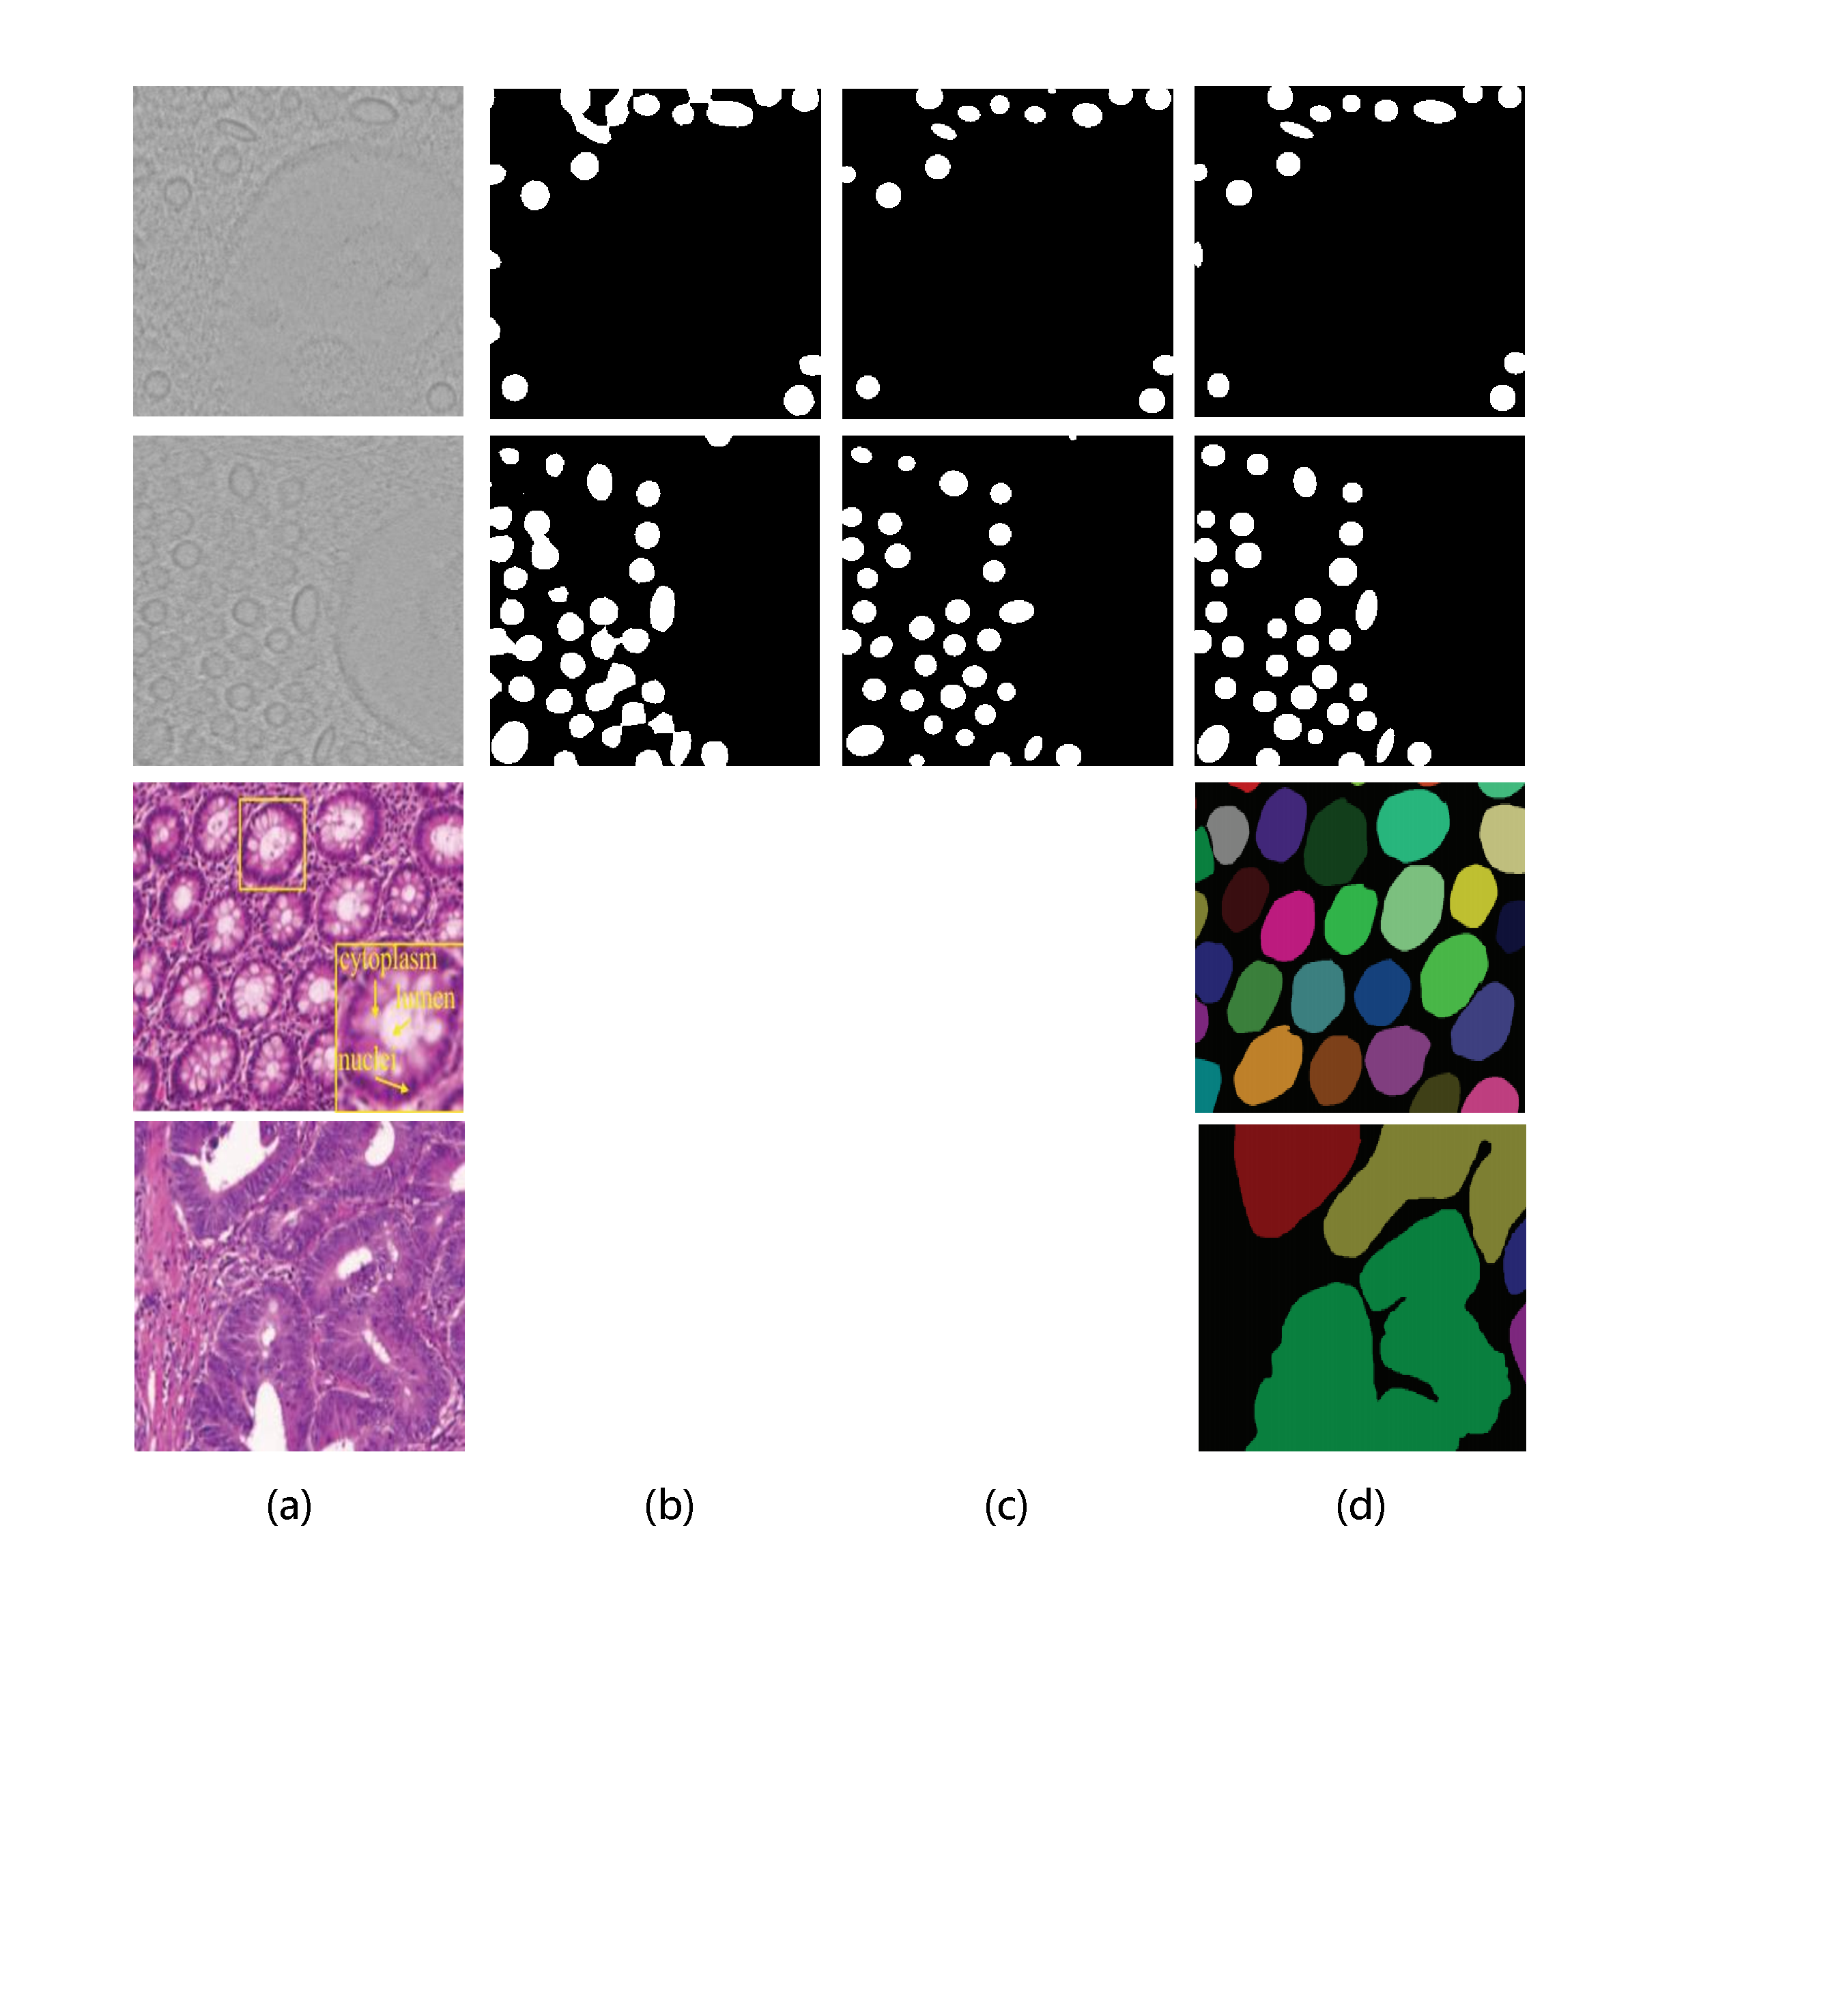
\includegraphics[width=3.3in]{figures/Fig1.pdf}
\end{center}
   \caption{Examples illustrating deficiency of existing methods for biomedical segmentation. First two rows are dense synaptic vesicle with regular shape, and bottom two rows are benign and malignant gland. (a) biomedical image; (b) results from DCAN \cxj{cite the reference}; (c) results from SCNN by incorporating prior shape constraint; (d) annotations by experts. \cxj{what are the blank areas for the last two rows?}}
   \label{FigImgs}
\end{figure}

\mdf{However, it is non-trivial to automatically segment biomedical images.} 
%[copy]However, there exists several challenges in these tasks.[copy]
First, biomedical images are usually noisy and of low contrast, because of deficient imaging techniques, as shown in Figure~\ref{FigImgs} (a).
%
Second, due to the compact and dense arrangement of majority membrane structures, it is hard to separate objects individually, which is known as the touching problem.
%
Third, as most deep neural architecture of biomedical images are based on fully convolutional networks~\cite{Long2015}, they inevitably suffer from poor localized object boundaries caused by large receptive fields and many pooling layers.
\cxj{put this sentence to the next paragraph?}



Recently, deep neural networks have demonstrated excellent performance in biomedical image segmentation with the use of fully convolutional networks \cite{Long2015,Dhungel2015,Ronneberger2015,Roth2015,Chen2015,Lieman-Sifry2017,Xu2016}.
\mdf{However, the pooling and downsampling layers in these networks make it inevitable to get poorly localized object boundaries.}
%
\mdf{To increase the boundary accuracy, many efforts have been made recently. A U-shaped deep network called U-net~\cite{Ronneberger2015} is proposed for biomedical image segmentation. By employing the skip connections between the contracting and expanding paths, context information can be directly propagated to higher resolution layers for detail preserving.
%
Several improvements of U-net were proposed soon afterwards. 
DeepVentricle~\cite{Lieman-Sifry2017}, which uses the same padding instead of valid padding, has been successfully used for cardiac segmentation.
Recently, DCAN~\cite{Chen2016a} integrates the complementary information of object regions and contours in a multi-task learning framework. \cxj{for more accurate boundaries?}
}
%
Although these methods achieved promising results in their segmentation tasks, they may fail to achieving satisfying performance in denser, smaller objects with regular shapes, as Figure~\ref{FigImgs} shows.
%
\mdf{More specifically}, segmenting synaptic vesicles in our task raises higher demand on localizing contour for each vesicles.



%
\comments{
For this reason, [copy]\cite{Ronneberger2015} proposed the U-net that designed a U-shaped deep convolutional network for biomedical image segmentation.[copy]
[copy]It uses skip connections between the contracting and expanding paths to directly propagate context information to higher resolution layers to preserve details.[copy]
Later, a UNet variant, DeepVentricle \cite{Lieman-Sifry2017}, has been used for cardiac segmentation, which used same padding instead of valid padding.
Further improvements have been shown in DCAN \cite{Chen2016a}, which [copy]investigates the complementary information of objects and contours under a multi-task learning framework.[copy]
Specially, [weak copy]DCAN simultaneously segment the object and separate the clustered objects into individual ones with the help of their contours[weak copy].}
%



\begin{figure*}\label{FigSCNN}
\begin{center}
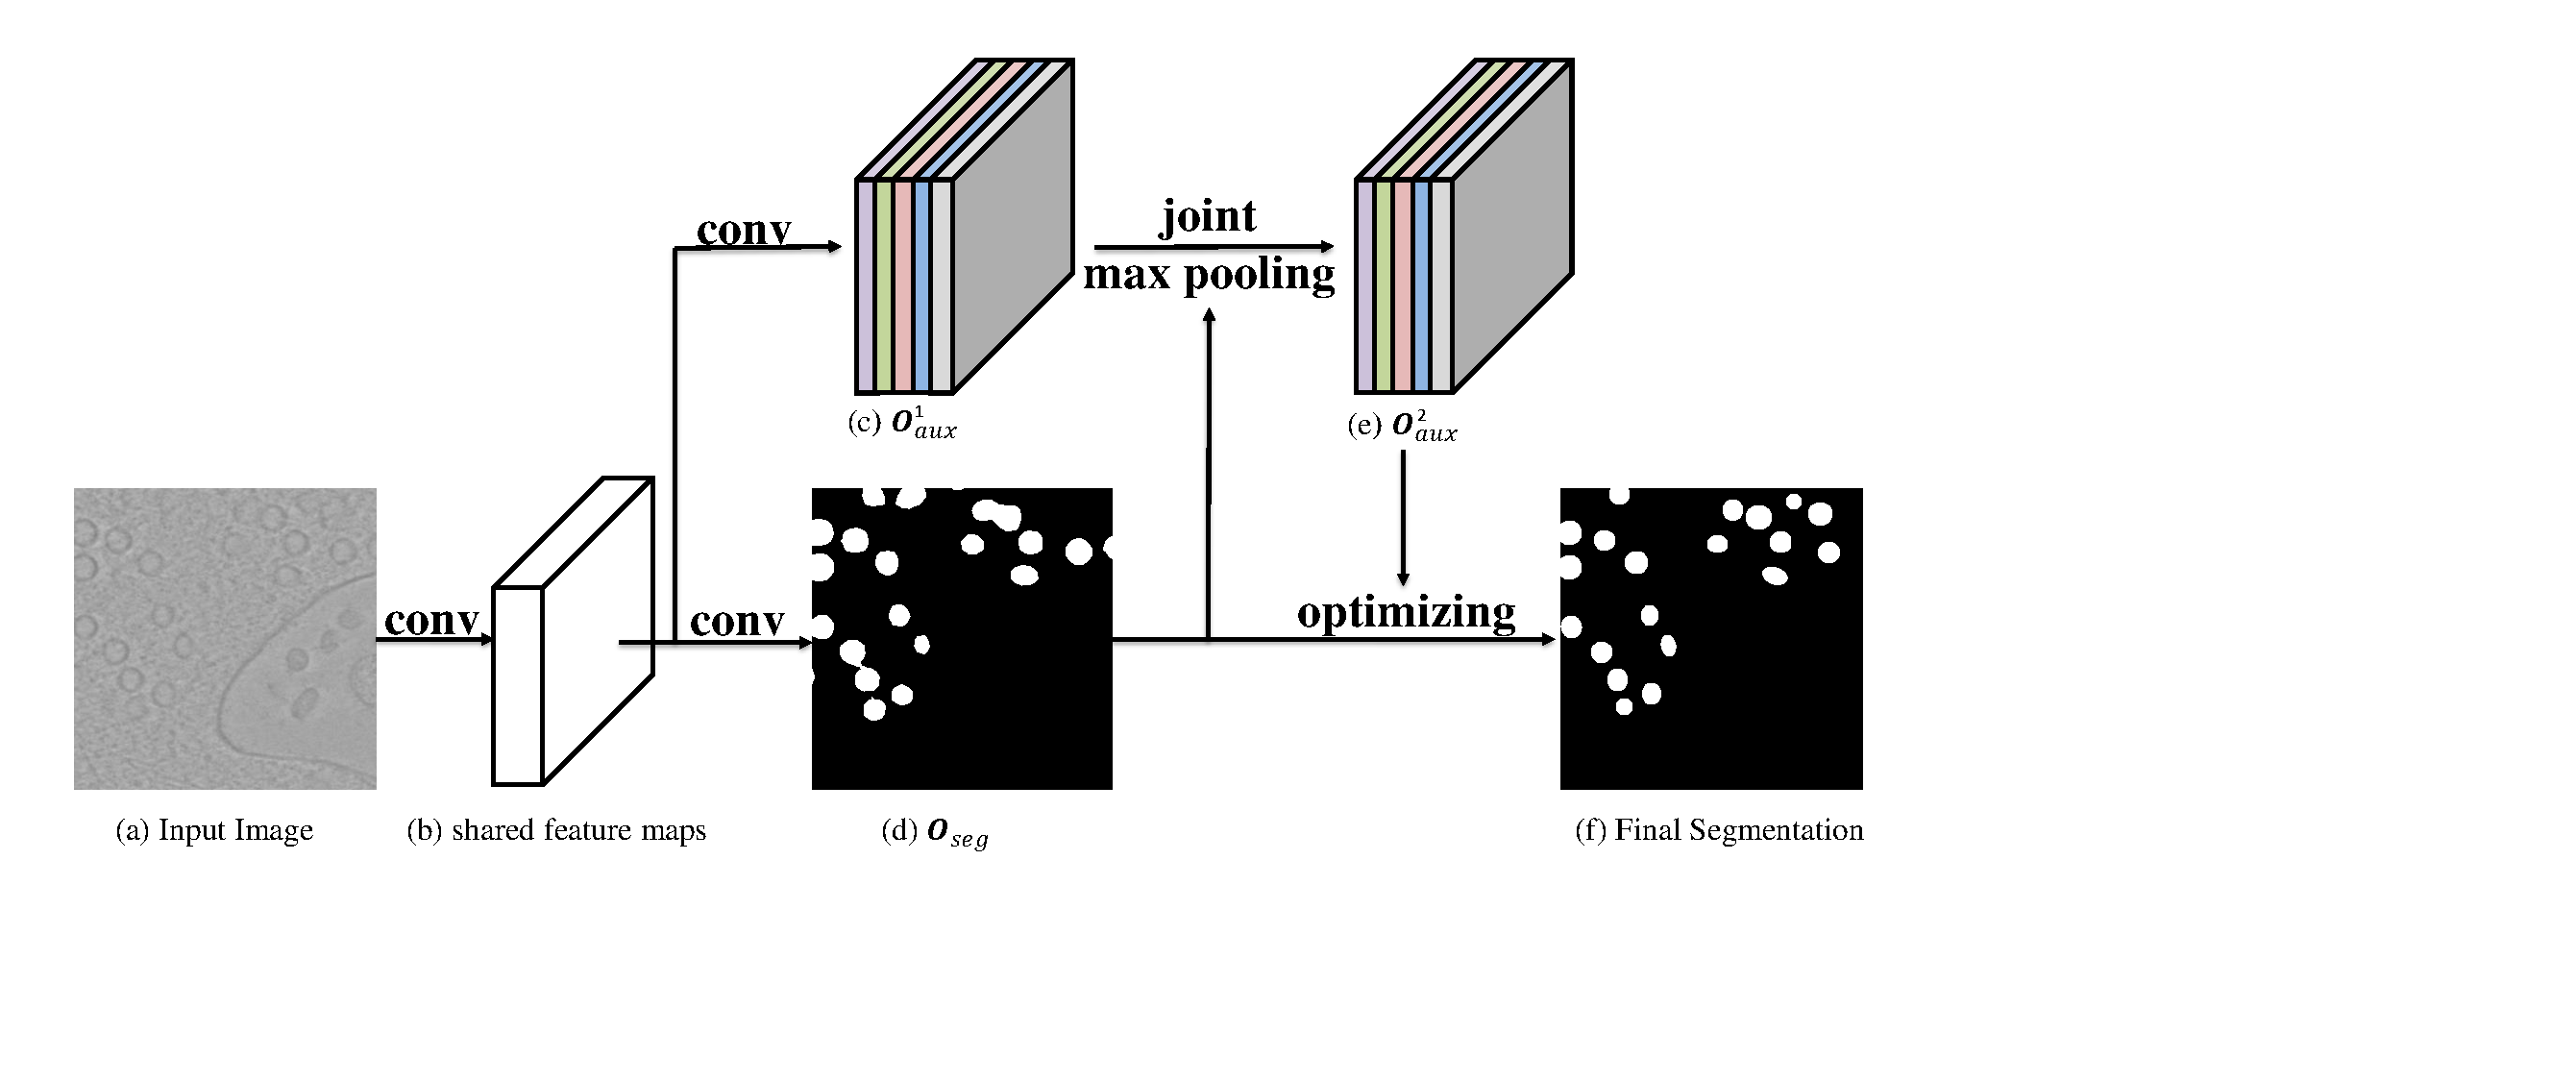
\includegraphics[width=6.8in]{figures/Fig2.pdf}
\end{center}
   \caption{Overview of our proposed scnet. Given an image (a), multi-task neural network simultaneously predict a coarse segmentation (d) and parameterized contour description (d) using shared feature maps (b).
   Then a joint max pooling is applied to pool (c) with (d) and output new parameterized contour description (e).
   Finally, segmentation (f) is obtained by optimizing coarse segmentation (d) with the parameterized contour description (e).}
\end{figure*}

In this paper, we propose the first \mdf{Shape-Constrained} neural network (SCNN) to segment dense objects by inherently incorporating prior shape knowledge into the network.
%while still accommodate serious shape deformation.
Similar with \cite{Chen2016a}, we formulate the network as a multi-task learning framework by simultaneously predicting a segmentation map and an auxiliary map.
%The auxiliary map, usually being contours map \cite{Chen2016a}, \cite{Chen2016}, \cite{Bertasius2016} ,is used to supplement complementary information for segmentation map.
Instead of predicting the contour probability map, as used in \cite{Chen2016a,Chen2016,Bertasius2016}, our SCNN learn\mdf{s} a parameterized description of the contour shape as \mdf{a} auxiliary map, which emphasizes more on \mdf{the} overall shape of objects.
%^In our framework, instead of directly predicting object contours, our SCNN learn the parameterized expression of contours, which emphasizes more on the overall shape of object.
%Especially, our parameterized contour expression can not only separate objects into individual ones, but also be embed in different shape constraint by defining different parameter composition.
The complementary information in parameterized contour description can not only separate objects into individual ones, but also optimizes the contours shape.
%
However since there existing some seriously deformable objects, contours shape \mdf{cannot} be parameterized uniformly and accurately.
To this end, we select a best representative shape as constraints and only modify segmentation predictions in ambiguous regions, where usually contains contours \cxj{what do you mean here?}, using the predicted parameterized contour description.
%In this way, most biomedical objects with regular shape, such as ellipse, are beneficial, while the segmentation of fractional deformable object are not obviously affected.

However, predicting parameterized contour description over the whole map is \mdf{significantly more challenging than generating} contour probability map.
\cxj{Why this is more difficult? what is the challenge?}
%Eespecially predictions within one object region it is hard to guarantee the predictions belonging to one object corresponding to an identical shape, and performance will drop obviously in contours area, which is the exact the area where we desire to modify the segmentation result.
Therefore, we proposed a novel joint max pooling (JMP) layer to only predict the contour description in center region of objects and fill the rest region with them.
Furthermore, JMP is designed as a trainable layer, of which the back propagation is benefit to both segmentation and parameterized contours description.
%Furthermore, it is designed as a trainable layer, which can be extended to any networks.
%Explicitly, the objectness map can be used to substitute the contours expressions belonging to one object region with the expression of the highest objectness score, which reduces the learning difficulties and improve the inference accuracy.
%And contours expression map will increase the penalties on objectness loss of the regions, where there exist disagreements between objectness prediction and parameterized countour prediction in trun.
%Our JMP can be implemented as a layer, which can be trained end-to-end and adopted to other multi-task networkds.

Overall, the contribution of this paper is three-fold:
\begin{enumerate}
	\item We first effectively incorporate shape constraint into deep neural networks.
	% for biomedical image segmentation.
	\item We propose a novel joint max pooling for benefiting both multi-task outputs.
	\item Our framework is applicable to a series of different tasks such as biomedical image segmentation, scent detection task and achieves the state-of-the-art performance.
\end{enumerate}


\comments{
3) achieving better performance on diverse biomedical segmentation tasks,
4) in experiments, we show that our method can be extended to scent detection task, which obtains the state of art performance
}
